\documentclass{beamer}
\include{graphicx}
\include{comment}
\usepackage{beamerthemesplit}
\title{PetaBricks}
\subtitle{Introduction}
\author{Jason Ansel}

\begin{document}

\frame{\maketitle}

\section[Outline]{}
\frame{\tableofcontents}

\section{Motivation}
\subsection{The Importance of Choice}
\frame{
\begin{itemize}
\item Claim: High performance parallel algorithms require a non-trivial composition of different algorithmic choices.
\item The optimal algorithmic choice may not always be clear to the programmer.
\item Optimal algorithmic choices vary by problem size, architecture, and data.
\item Search over algorithmic choices can be automated.
\end{itemize}
}

\subsection{Simple Example Problem}
\frame{
\begin{itemize}
\item Sort on a cluster of multi-core processors:
\item The optimal solution {\bf might} be:
  \begin{itemize}
  \item Merge-sort at the cluster level (for load balancing)
  \item Quick-sort at the node level
  \item Insertion sort for very small lists
  \end{itemize}
\item For such a simple example it is easy for the human to guess this.
\end{itemize}
}

\subsection{Motivating Example Problem}
\frame{
\begin{itemize}
\item Poisson's equation.  A heat source is applied to the edges of matrix, find the steady state temperature for the matrix.
\item Can be solved many ways:
  \begin{itemize}
  \item MultiGrid
  \item SOR
  \item DST -> Mask-> Inverse DST
  \item LU
  \item ... 
  \end{itemize}
\end{itemize}
}

\frame{
\begin{itemize}
\item Choice space is large:
  \begin{itemize}
  \item MultiGrid -- {\em is recursive}
    \begin{itemize}
    \item MultiGrid
    \item SOR
    \item DST
    \item LU
    \end{itemize}
  \item SOR -- {\em has its own choices}
  \item DST -- {\em has its own choices}
  \item LU  -- {\em has its own choices}
  \end{itemize}
\end{itemize}
}


\frame{
\begin{itemize}
\item Choice space is {\bf really} large:
  \begin{itemize}
  \item Algorithmic choices
    \begin{itemize}
    \item \small Which algorithm(s)? When to switch?
    \end{itemize}
  \item Iteration order choices
    \begin{itemize}
    \item\small
      Columns? Rows? Blocks? How big?
    \end{itemize}
  \item Parallelism strategy choices
    \begin{itemize}
    \item\small
    Task? Data? Pipeline? How scheduled? Granularity?
    \end{itemize}
  \item Storage choices 
   \begin{itemize}
    \item\small
    Row major? Column major? Blocked? Transpose first? Storage/parallelism trade off.
    \end{itemize}
  \end{itemize}
\end{itemize}
}

\section{Language Design}
\frame{
\frametitle{A Bad Way to Represent Choice}
\begin{itemize}
\item A possible design adds a keyword:
  \begin{itemize}
  \item\small\tt either\{ A=foo(); \}or\{ A=bar(); \} 
  \end{itemize}
\item We did {\bf not} choose this:
  \begin{itemize}
  \item Hard to analyze 
  \item Hard to parallelize 
  \item Implicit choices (ie: blocking, storage, etc) are hard to represent 
  \end{itemize}
\end{itemize}
}

\subsection{Design Goals}
\frame{
\begin{itemize}
\item Design goals:
  \begin{itemize}
  \item Choices are represented naturally
  \item Easy to analyze
  \item Implicitly parallel
  \item Compiler is given a lot of freedom
  \begin{itemize}
    \item No outer sequential control flow
  \end{itemize}
  \end{itemize}
\end{itemize}
}

\subsection{Language Primitives}
\frame{
\begin{itemize}
\item Basic language element: {\bf Transform}
  \begin{itemize}
  \item Specifies from/through/to matrices 
  \end{itemize}
\end{itemize}
\begin{center}
\resizebox{\textwidth}{!}{
\includegraphics{transform}
}
\end{center}
}

\frame{
\begin{itemize}
\item Basic language element: {\bf Transform}
  \begin{itemize}
  \item Sizes are expressed symbolically
  \end{itemize}
\end{itemize}
\begin{center}
\resizebox{\textwidth}{!}{
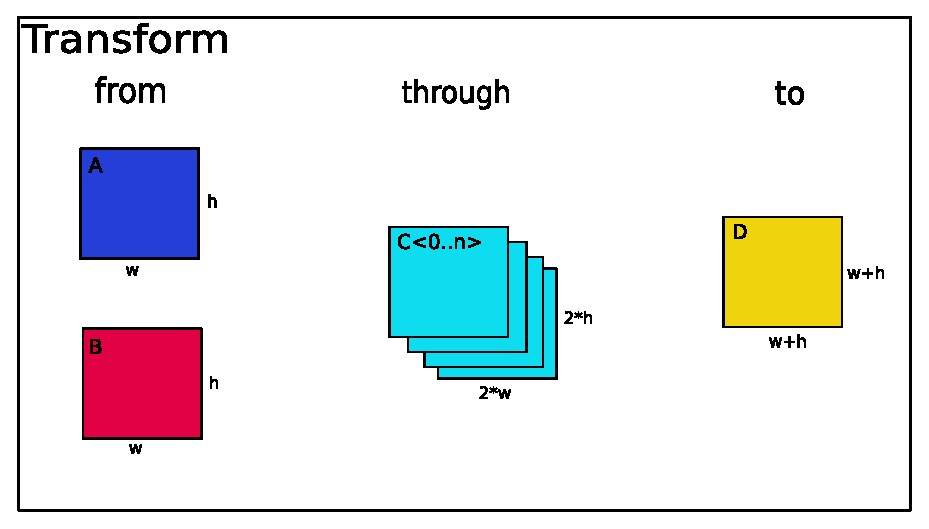
\includegraphics{transform-sizes}
}
\end{center}
}

\frame{
  \begin{itemize}
  \item Rules allow matrix elements and regions to be computed
  \end{itemize}
\begin{center}
\resizebox{\textwidth}{!}{
\includegraphics{transform-rules}
}
\end{center}
}

\frame{
  \begin{itemize}
  \item More on Rules:
    \begin{itemize}
    \item Rules explicitly list their dependencies in the from/to/through matrices 
    \item Work on either single elements or regions
    \item Can recursively call other transforms
    \item Use symbolic coordinates.
    { \small IE: from {\tt A.cell(x+1, y+1)} and {\tt B.cell(x-1, y-1)} compute {\tt C.cell(x,y)}}
    \end{itemize}
  \end{itemize}
}



\subsection{Example Code}

\begin{frame}[fragile]
\begin{itemize}
\item Now for some code:
{\small
\begin{verbatim}
 transform MatrixAdd
 from A[w,h], B[w,h] 
 to AB[w,h]
 {
   // just a single rule
   AB.cell(x,y) from( A.cell(x,y) a
                    , B.cell(x,y) b){
     return a+b;
   }
 }
\end{verbatim}
}
\end{itemize}
\end{frame}

\begin{frame}[fragile]
\begin{minipage}{\textwidth}
{\footnotesize
\begin{verbatim}
 transform Sort 
 from IN[n]
 to OUT[n]
 {
   // recursive case
   OUT from( IN.region(0,   n/2) left
           , IN.region(n/2, n)   right){
     return Merge( Sort(left), Sort(right) );
   }
   // base case
   OUT from( IN i ){ ... }
 }
\end{verbatim}
}
\end{minipage}
\end{frame}

\section{Internals}
\subsection{Infrastructure Diagram}
\frame{
\begin{center}
\resizebox{\textwidth}{!}{
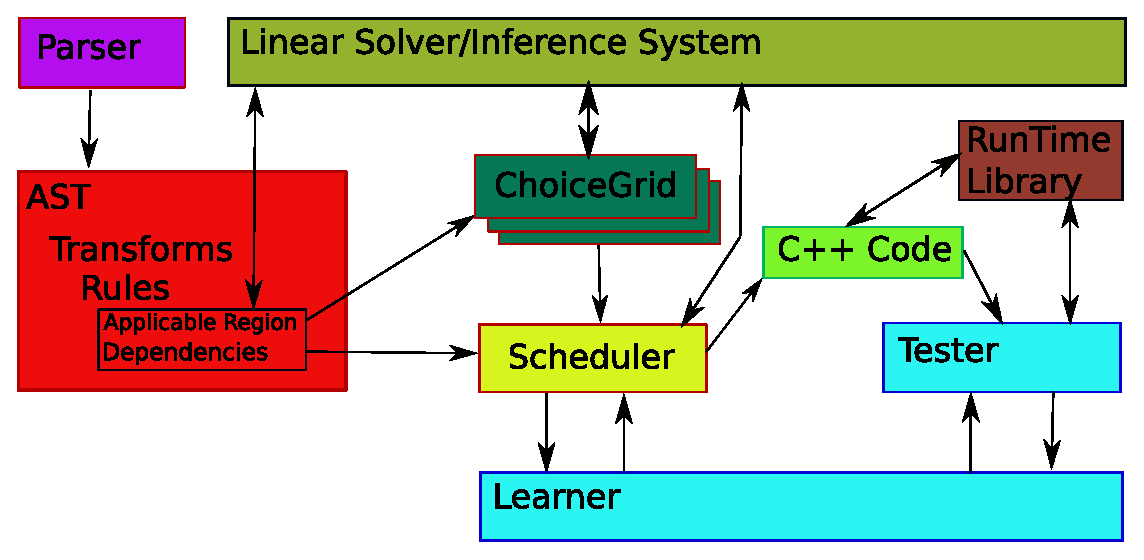
\includegraphics{internals}}
\end{center}
}

\frame{
\begin{center}
\resizebox{\textwidth}{!}{
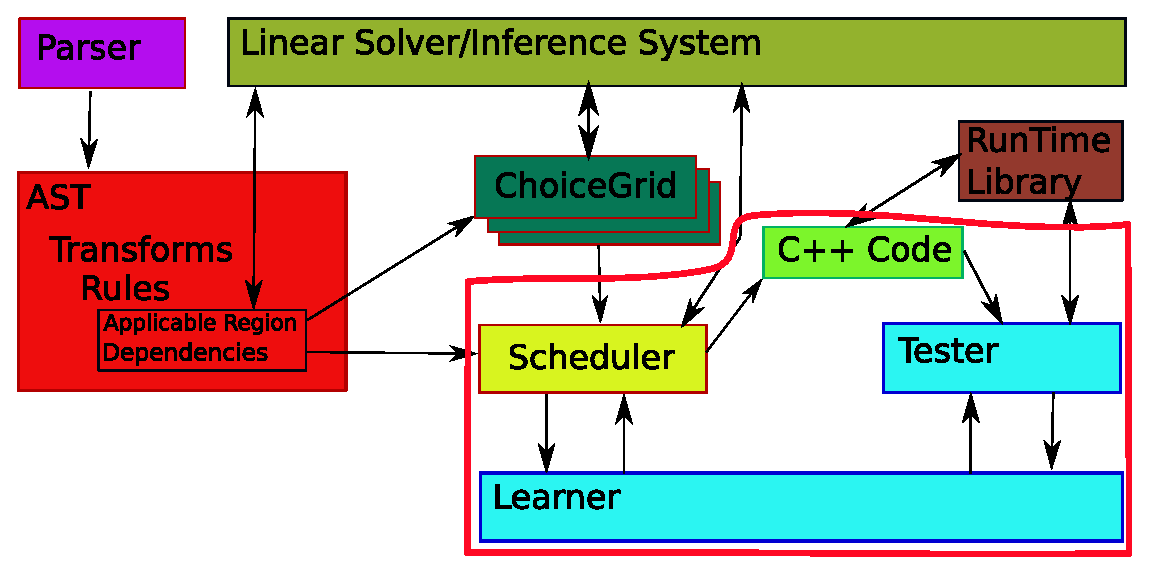
\includegraphics{internals2}}
\end{center}
}

\end{document}
